\documentclass{article}

\usepackage{amsfonts}
\usepackage{amsmath}
\usepackage[dvips]{epsfig}
\usepackage[dcu]{harvard}
\usepackage{dcolumn}
\usepackage{shortvrb}
\usepackage{parskip}
\usepackage{multicol}

\sloppy
\parindent0em
\topmargin-1.5cm \textheight23cm \textwidth15cm
\oddsidemargin0.5cm

\MakeShortVerb{\#}

\begin{document}
\title{Bayesian semiparametric regression based on MCMC techniques: A tutorial}
\author{Thomas Kneib, Stefan Lang and Andreas Brezger\\ [.25cm]
\normalsize Department of Statistics, University of Munich. }
\maketitle

\begin{abstract}
This tutorial demonstrates the usage of {\it BayesX} for analysing
Bayesian semiparametric regression models based on MCMC
techniques. As an example we consider data on undernutrition of
children in Zambia. The tutorial is designed to be self-contained
and describes all features of {\it BayesX} in detail, that will be
needed throughout the tutorial. Therefore it may also serve as a
first introduction into the general usage of {\em BayesX}.
\end{abstract}

\tableofcontents

\newpage
\section{Introduction}\label{data}

This tutorial demonstrates the usage of {\it BayesX} for analysing
Bayesian semiparametric regression models based on MCMC
techniques. As an example we consider data on undernutrition of
children in Zambia. This data has already been analysed in Kandala
et al. (2001) \nocite{kanlan01} and we will use the same model
that has been developed there. Since our focus is on demonstrating
how regression models can be estimated in {\em BayesX}, we do not
discuss or interpret the estimation results but simply give the
commands to produce them.

The main focus in this tutorial is on full Bayesian inference based
on MCMC-techniques. {\it BayesX} also supports the estimation of
semiparametric regression models in an empirical Bayes context based
on mixed model methodology. An advantage of the the full Bayesian
approach is, that it can deal with massive data sets while the
empirical Bayes approach is limited to data sets with medium sample
size. On the other side, questions about the convergence of MCMC
samples or sensitivity on hyperparameters do not arise in the
empirical Bayes approach. Furthermore, this approach may be much
faster in situations with a relatively small number of regression
parameters and non-normal responses. A comparison of both approaches
in a simulation study has shown, that the empirical Bayes approach
yields somewhat better point estimates, especially for Bernoulli
distributed response, see Fahrmeir, Kneib and Lang
(2004).\nocite{fahkne04}

A second tutorial, dealing with the empirical Bayes approach is
available from the tutorials section of the {\it BayesX}-homepage.
All tutorials are designed to be self-contained and describe all
features of {\it BayesX} in detail, that will be needed throughout
the tutorial. Users who are already familiar with the usage of
{\it dataset} and {\it map objects} may therefore skim through
sections \ref{usage}-\ref{maps}.

The theoretical background of Bayesian semiparametric regression
will not be described in this tutorial. Chapter 7 of the manual may
serve as an introduction, full details about the estimation
techniques for the full Bayesian approach can be found in Fahrmeir
and Lang (2001a,2001b),\nocite{fahlan01a}\nocite{fahlan01b} Lang and
Brezger (2004) and Brezger and Lang
(2005).\nocite{lanbre04}\nocite{lanbre05} Survival models are
treated in Hennerfeind, Brezger and Fahrmeir (2003)\nocite{henfah03}
and Fahrmeir and Hennerfeind (2003)\nocite{fahhen03}, Count data
regression is covered in Fahrmeir and Osuna (2003)\nocite{fahosu03}.

\section{Description of the data set}

Undernutrition among children is usually determined by assessing
the anthropometric status of a child relative to a reference
standard. In our example undernutrition is measured by stunting or
insufficient height for age, indicating chronic undernutrition.
Stunting for a child $i$ is determined using a Z-score which is
defined as
\[Z_i = \frac{AI_i-MAI}{\sigma}\]
where $AI$ refers to the child`s anthropometric indicator (height
at a certain age in our example), MAI refers to the median of the
reference population and $\sigma$ refers to the standard deviation
of the reference population.

The main interest is on modelling the dependence of undernutrition
on covariates including the age of the child, the body mass index
of the child`s mother, the district the child lives in and some
further categorial covariates. Table \ref{zambiavar} gives a
description of the variables that we will use in our model.

{\footnotesize
\begin{table}[ht]
\begin{center}
\begin{tabular}{|l|p{12.5cm}|}
 \hline
 {\bf Variable} & {\bf Description}\\
 \hline
 $hazstd$ & standardised Z-score of stunting\\
 $bmi$ & body mass index of the mother\\
 $agc$ & age of the child in months\\
 $district$ & district where the child lives\\
 $rcw$ & mother`s employment status with categories "working" (= 1) and "not working" (= $-1$)\\
 $edu1/2$ & mother`s educational status with categories "complete primary but incomplete secondary" ($edu1=1$), "complete secondary or higher" ($edu2=1$) and "no education or incomplete primary" ($edu1=edu2=-1$)\\
 $tpr$ & locality of the domicile with categories "urban" (= 1) and "rural" (= $-1$)\\
 $sex$ & gender of the child with categories "male" (= 1) and
 "female" (= $-1$)\\
 \hline
\end{tabular}
{\it\caption{Variables in the undernutrition data set.
\label{zambiavar}}}
\end{center}
\end{table}}

\section{Getting started}\label{usage}

After having started {\em BayesX}, a main window with four
sub-windows appears on the screen. These are a {\em command
window} for entering and executing code, an {\em output window}
for displaying results, a {\em review window} for easy access to
past commands, and an {\em object browser} that displays all
objects currently available.

{\em BayesX} is object oriented although the concept is limited,
i.e. inheritance and other concepts of object oriented languages
like C++ or S-plus are not supported. For every object type a
number of object-specific methods may be applied to a particular
object. The syntax for generating a new object in {\em BayesX} is
\medskip

{\tt> }{\em objecttype objectname}
\medskip

where {\em objecttype} is the type of the object, e.g. {\tt
dataset}, and {\em objectname} is the name to be given to the new
object.

The rest of the tutorial is separated in seven parts dealing with
the different steps of estimating a regression model. In section
\ref{datasets} we create a {\em dataset object} to incorporate,
handle and manipulate the data. We will also give a brief
description of some methods that may be applied to {\em dataset
objects}. Since we want to estimate a spatial effect of the
district in which a child lives, we need the boundaries of the
districts to compute the neighbourhood information of the map of
Zambia. This information will be stored in a {\em map object}.
Section \ref{maps} describes how to create and handle these
objects. Estimation of the regression model is carried out in
section \ref{regression} using a {\em bayesreg object}. The next
two sections describe how to visualise the estimation results and
how to customise the obtained graphics. Section \ref{postest}
describes post estimation commands which can be used to
investigate the sampling paths and the autocorrelation functions
of the estimated parameters. In a last section we perform a
sensitivity analysis to assess the impact of hyperparameter
choices on our estimation results.

If you have not done so yet, please download the data set and the
{\it boundary file} associated with this tutorial now. You may
also want to download the batch file containing the commands used
in the following sections. Please note, that paths within these
commands must be changed according to the storage location of the
corresponding files on your hard disk.

\section{Reading data set information}\label{datasets}

In a first step we read the available data set information into
{\it BayesX}. Therefore we create a {\it dataset object} named
#d#:

#> dataset d#

We store the data in #d# using the method #infile#:

#> d.infile, maxobs=5000 using c:\data\zambia.raw#

Note, that we assume the data to be provided in the external file
#c:\data\zambia.raw#. The first few lines of this file look like
this:

{\footnotesize
 hazstd bmi agc district rcw edu1 edu2 tpr sex\\
 0.0791769 \,\, 21.83 \,\, 4 \,\, 81 \,\, -1 \,\, 1 \,\, 0 \,\, 1 \,\, -1\\
 -0.2541965 \,\, 21.83 \,\, 26 \,\, 81 \,\, -1 \,\, 1 \,\, 0 \,\, 1 \,\, -1\\
 -0.1599823 \,\, 20.43 \,\, 56 \,\, 81 \,\, 1 \,\, -1 \,\, -1 \,\, 1 \,\, 1\\
 0.1733911 \,\, 22.27 \,\, 6 \,\, 81 \,\, -1 \,\, 0 \,\, 1 \,\, 1 \,\, 1}

In our example the file contains the variable names in the first
line. Therefore it is not necessary to specify them in the
#infile# command. If the file contained only the data without
variable names, we would have to supply them after the keyword
#infile#:

 #> d.infile hazstd bmi agc district rcw edu1 edu2 tpr sex, maxobs=5000#
 #  using c:\data\zambia.raw#


Option #maxobs# can be used to speed up the execution time of the
#infile# command. If #maxobs# is specified, {\it BayesX} allocates
enough memory to store all the data while the total amount of
required memory is unknown in advance if #maxobs# remains
unspecified. For larger data sets this may cause {\it BayesX} to
start reading the data set information several times because the
currently allocated memory is exceeded. However, this is only
meaningful for larger data sets with more than 10,000 observations
and could therefore be omitted in our example.

A second option that may be added to the {\tt infile} command is the
{\tt missing} option to indicate missing values. Specifying for
example '{\tt missing = M}' defines the letter '{\tt M}' as an
indicator for a missing value. The default for missing values are a
period '.' and '{\tt NA}' (which remain valid indicators for missing
values even if an additional indicator is defined by the {\tt
missing} option).

After having read in the dataset information we can inspect the
data visually. Executing the command

#> d.describe#

opens an {\it Object-Viewer} window containing the data in form of
a spreadsheet (see Figure \ref{screenshot}). This can also be
achieved by double-clicking on the {\it dataset object} in the
{\it object browser}.

\vspace{1cm}

\begin{figure}[ht]
\begin{center}
\epsfig{file=grafiken/screenshot2.eps,scale=0.5} {\it\caption{A
screenshot of the dataset.\label{screenshot}}}
\end{center}
\end{figure}

Further methods allow to examine the variables in the {\it dataset
object}. For a categorial variable, e.g. $sex$, the #tabulate#
command may be used to produce a frequency table:

#> d.tabulate sex#

resulting in

\begin{verbatim}
Variable: sex

          Value       Obs           Freq            Cum
             -1      2451         0.5057         0.5057
              1      2396         0.4943              1
\end{verbatim}

being printed in the {\it output window}. For continuous variables
the #descriptive# command prints several characteristics of the
variable in the {output window}. E.g., executing

#> d.descriptive bmi#

leads to

\begin{verbatim}
   Variable    Obs        Mean      Median         Std         Min         Max
        bmi   4847   21.944349        21.4   3.2879659        12.8       39.29
\end{verbatim}

\section{Map objects}\label{maps}

In the following we want to estimate a spatially correlated effect
of the district in which a child lives. Therefore we need the
boundaries of the districts in Zambia to compute the neighbourhood
information of the map of Zambia. We therefore create a {\it map
object}

#> map m#

and read in the boundaries using the #infile# command of {\it map
objects}:

#> m.infile using c:\data\zambia.bnd#

Having read in the boundary information, {\it BayesX}
automatically computes the neighbourhood matrix of the map.

The file following the keyword #using# is assumed to contain the
boundaries in form of closed polygons. To give an example we print
a small part of the boundary file of Zambia. The map corresponding
to the section of the boundary file can be found in Figure
\ref{zambia52}.

\footnotesize

\hspace{1cm}  $\vdots$

 "52",48\\
 28.080507,-12.537530\\
 28.083376,-12.546980\\
 28.109501,-12.548961\\
 28.134972,-12.566787\\
 28.154797,-12.585320\\
 28.165771,-12.593912\\
 28.165771,-12.593912\\
 28.160769,-12.609917\\
 28.152800,-12.633824\\
 28.144831,-12.657733\\
 28.132877,-12.677656\\
 28.120922,-12.701565\\
 28.120922,-12.717505\\
 28.120922,-12.741411\\
 28.116938,-12.761335\\
 28.108969,-12.777274\\
 28.100998,-12.793213\\
 28.089045,-12.817122\\
 28.085060,-12.837045\\
 28.081076,-12.856968\\
 28.081076,-12.876892\\
 28.080862,-12.884153\\
 28.080862,-12.884153\\
 28.076630,-12.879521\\
 28.031454,-12.881046\\
 27.974281,-12.884675\\
 27.910725,-12.878692\\
 27.686228,-12.880120\\
 27.665676,-12.854732\\
 27.653563,-12.818301\\
 27.639263,-12.759848\\
 27.648254,-12.699927\\
 27.662464,-12.680613\\
 27.662464,-12.680613\\
 27.666534,-12.675080\\
 27.703260,-12.679779\\
 27.752020,-12.695455\\
 27.797932,-12.702188\\
 27.836775,-12.707567\\
 27.867813,-12.699892\\
 27.902308,-12.667418\\
 27.922668,-12.630853\\
 27.943035,-12.596350\\
 27.963434,-12.571486\\
 27.983179,-12.563844\\
 28.016331,-12.554779\\
 28.070650,-12.542199\\
 28.080507,-12.537530\\

\hspace{1cm} $\vdots$

\normalsize

\vspace{0.3cm}

For each region of the map the boundary file must contain the
identifying name of the region, the polygons that form the
boundary of the region, and the number of lines the polygon
consists of. The first line always contains the region code
surrounded by quotation marks and the number of lines the polygon
of the region consists of. The code and the number of lines must
be separated by a comma. The subsequent lines contain the
coordinates of the straight lines that form the boundary of the
region. The straight lines are represented by the coordinates of
their end points. Coordinates must be separated by a comma. Note
that the first and the last point must be identical (see the
example above) to obtain a closed polygon. Compare chapter 5 of
the complete manual for a detailed description of some special
cases, e.g. regions divided into subregions.

\begin{figure}[h]
\centering

\includegraphics [scale=0.3]{grafiken/zambia52.ps}
\caption{\label{zambia52} Corresponding graph of the section of
the boundary file}
\end{figure}

{\it Map objects} may be visualised using method #describe#:

#> m.describe#

resulting in the graph shown in Figure \ref{zambiamap}.
Additionally, #describe# prints further information about the {\it
map object} in the {\it output window} including the name of the
object, the number of regions, the minimum and maximum number of
neighbours and the bandwidth of the corresponding adjacency or
neighbourhood matrix:

\begin{verbatim}
  MAP m
  Number of regions: 54
  Minimum number of neighbors: 1
  Maximum number of neighbors: 9
  Bandsize of corresponding adjacency matrix: 24
\end{verbatim}

\begin{figure}[ht]
\begin{center}
\epsfig{file=grafiken/zambia.ps,scale=0.35} {\it\caption{The
districts within Zambia.\label{zambiamap}}}
\end{center}
\end{figure}


The numerical complexity associated with the estimation of
structured spatial effects using MCMC techniques depends
essentially on the structure of the neighbourhood matrix. Often
the geographical information stored in a boundary file does not
represent the ''ideal'' ordering (as regards to the estimation
problem) of the districts or regions. Therefore it may be useful
to reorder the map using method #reorder#:

#> m.reorder#

Usually reordering results in a smaller bandwidth although the
bandwidth is not the criterion that is minimised by #reorder#.
Instead the {\it envelope} of the neighbourhood matrix is
minimised (compare George and Liu 1981) \nocite{geoliu81}.

In order to avoid reordering the {\it map object} every time you
start {\it BayesX} it is useful to store the reordered version in
a separate file. This can be achieved using the #outfile# command
of {\it map objects}:

#> m.outfile, replace using c:\data\zambiasort.bnd#\\

The reordered map is now stored in the given file. Note, that
specifying the option #replace# allows {\it BayesX} to overwrite
an existing file with the same name. Without this option an error
message would be raised if the given file is already existing.

Reading the boundary information from an external file and
computing the neighbourhood matrix may be a computationally
intensive task if the map contains a large number of regions or if
the polygons are given in great detail. To avoid doing these
computation in every $BayesX$ session, we store the neighbourhood
information in a so-called {\it graph file} using method #outfile#
together with the #graph# option:

#> m.outfile, replace graph using c:\data\zambiasort.gra#\\

A graph file stores the nodes and the edges of a graph $G =
(N,E)$, see for example George and Liu (1981, Ch. 3) for a first
introduction into graph theory. A graph is a convenient way of
representing the neighbourhood structure of a geographical map.
The nodes of the graph correspond to the region codes. The
neighbourhood structure is represented by the edges of the graph.
In some situations it may be useful to define weights associated
with the edges of a graph which can be be stored in the {\em graph
file} as well.

We now describe the structure of a graph file as it is expected by
{\em BayesX}. The first line of a {\em graph file} must contain
the total number of nodes of the graph. In the remaining lines,
the nodes of the graph together with their edges and associated
weights are specified. One node corresponds to three consecutive
lines. The first of the three lines must contain the name of the
node, which may simply be the name of a geographical region. In
the second line the number of edges of that particular node is
given. The third line contains the corresponding edges of the
node, where an edge is given by the index of a neighbouring node.
The index starts with zero. For example, if the fourth and the
seventh node/region in the {\em graph file} are
connected/neighbours, the edge index for the fourth node/region is
6 and for the seventh node/region 3.

We illustrate the structure of a graph file with an example. The
following few lines are the beginning
of the graph file corresponding to the reordered map of Zambia: \\

\footnotesize

 57\\
 87\\
 1\\
 5\\
 76\\
 3\\
 9 8 7\\
 67\\
 2\\
 10 9\\

\hspace{1cm} $\vdots$

\normalsize

\vspace{0.5cm}

The first line specifies the total number of nodes, in the present
example 57 nodes. The subsequent three lines correspond to the
node with name '87', which is the first region in the reordered
map of Zambia. Region '87' has 1 neighbour, namely the sixth node
appearing in the graph file. Once again, note that the index
starts with zero, i.e. 0 corresponds to the first node, 1
corresponds to the second node and so on. Lines 5 to 7 in the
example correspond to node '76' and its three neighbours and lines
8 to 10 correspond to node '67'.

In a graph file it is also possible to specify weights associated
with the edges of the nodes. Since in the preceding example no
weights are explicitly specified, all weights are automatically
defined to be equal to one. Nonequal weights are specified in the
graph file by simply adding them following the edges of a
particular node.
An example of the beginning of a graph file with weights is given below: \\

\footnotesize

 57\\
 87\\
 1\\
 5 1.44172\\
 76\\
 3\\
 7 8 9 0.707424 1.3816 0.682372\\
 67\\
 2\\
 9 10 1.67424 0.8406\\

\hspace{1cm} $\vdots$

\normalsize

\vspace{0.5cm}

Here the edge of the first node '87' has weight 1.44172, the edges
of the second node have weights 0.707424, 1.3816 and 0.682372.

Note, that graph files allow the estimation of more general Markov
random fields. While the polygons stored in a {\em boundary file}
represent geographical information, the nodes and edges of a graph
may define arbitrary neighbourhood structures. For example, the
definition of 3 dimensional Markov random fields representing
space-time interactions is possible.

To see how storing maps in {\it graph files} affects the
computation time of the #infile# command, we create a second {\it
map object} and read in the information from the graph file.
Again, we have to specify the keyword #graph#:

\begin{verbatim}
> map m1
> m1.infile, graph using c:\data\zambiasort.gra
\end{verbatim}

As you should have noticed, reading geographical information from
a {\it graph file} is usually much faster than reading from a {\it
boundary file}. However, using {\it graph files} also has a
drawback. Since they do no longer contain the full information on
the polygons forming the map, we can not visualise a {\it map
object} created from a {\it graph file}. Trying to do so

#> m1.describe#

raises an error message. This implies, that visualising estimation
results of spatial effects can only be based on {\it map objects}
created from {\it boundary files}, although estimation can be
carried out using {\it graph files}. Since we will work with the
{\it map object} #m# in the following, we delete #m1#:

#> drop m1#

\section{Bayesian semiparametric regression}\label{regression}

To estimate a regression model using MCMC techniques we first
create a {\it bayesreg object}:

#> bayesreg b#

By default estimation results are written to the subdirectory
#output# of the installation directory. In this case the default
filenames are composed of the name of the {\it bayesreg object}
and the type of the specific file. Usually it is more convenient
to store the results in a user-specified directory. To define this
directory we use the #outfile# command of {\it bayesreg objects}:

#> b.outfile = c:\data\b#

Note, that #outfile# does not only specify a directory but also a
base filename (the character 'b' in our example). Therefore
executing the command above leads to storage of the results in the
directory '#c:\data#' and all filenames start with the character
'b'. Of course the base filename may be different from the name of
the {\it bayesreg object}.

In addition to parameter estimates {\it BayesX} also gives
acceptance rates for the different effects and some further
information on the estimation process. In contrast to parameter
estimates this information is not stored automatically but is
printed in the {\it output window}. Therefore it is useful to
store the contents of the {\it output window}. This can be
achieved automatically by opening a {\it log file} using the
#logopen# command

#> logopen, replace using c:\data\logmcmc.txt#

After opening a {\it log file}, every information written to the
output window is also stored in this file. Option #replace# allows
{\it BayesX} to overwrite an existing file with the same name as the
specified {\it log file}. Without #replace# results are appended to
an existing file.

The model presented in Kandala et al. (2001) is given by the
following semiparametric predictor:
\[\eta=\gamma_0+\gamma_1rcw+\gamma_2edu1+\gamma_3edu2+\gamma_4tpr+\gamma_5sex+f_1(bmi)+f_2(agc)+f^{str}(district)+f^{unstr}(district)\]
The two continuous covariates {\em bmi} and {\em agc} are assumed to
have a possibly nonlinear effect on the Z-score and are therefore
modelled nonparametrically (as P-splines with second order random
walk prior in our example). The spatial effect of the district is
split up into a spatially correlated part $ f^{str}(district)$ and
an uncorrelated part $f^{unstr}(district)$, see Fahrmeir and Lang
(2001b) \nocite{fahlan01b} for a motivation. The correlated part is
modelled by a Markov random field prior, where the neighbourhood
matrix and possible weights associated with the neighbours are
obtained from the {\it map object} #m#. The uncorrelated part is
modelled by an i.i.d. Gaussian effect.

To estimate the model we use method #regress# of {\em bayesreg
objects}:
\begin{verbatim}
> b.regress hazstd = rcw + edu1 + edu2 + tpr + sex + bmi(psplinerw2)
  + agc(psplinerw2) + district(spatial,map=m) + district(random),
  family=gaussian iterations=12000 burnin=2000 step=10 predict using d
\end{verbatim}

Options {\tt iterations}, {\tt burnin} and {\tt step} define
properties of the MCMC-algorithm. The total number of MCMC
iterations is given by {\tt iterations} while the number of burn in
iterations is given by {\tt burnin}. Therefore we obtain a sample of
10000 random numbers with the above specifications. Since, in
general, these random numbers are correlated, we do not use all of
them but thin out the Markov chain by the thinning parameter {\tt
step}. Specifying {\tt step=10} as above forces {\em BayesX} to
store only every 10th sampled parameter which leads to a random
sample of length 1000 for every parameter in our example.

Note, that the choice of {\tt iterations} also affects computation
time. On a 2.4 GHz PC estimation of our model took about 1 minute
and 5 seconds, which is rather fast in regard of the complexity of
the model.

If option {\tt predict} is specified, samples of the deviance, the
effective number of parameters $p_D$, and the deviance information
criteria $DIC$ of the model are computed, see Spiegelhalter et al.
(2002).\nocite{spibes02} In addition, estimates for the linear
predictor and the expectation of every observation are obtained.

In the following we reproduce the content of the {\em output
window} to make the user familiar with the estimation results
produced by {\em BayesX}:

\footnotesize
\begin{verbatim}
ESTIMATION RESULTS:

  Predicted values:

  Estimated mean of predictors, expectation of response and
  individual deviances are stored in file
  c:\data\b_predictmean.raw

  Estimation results for the deviance:

  Unstandardized Deviance (-2*Loglikelihood(y|mu))

  Mean:             12688.959
  Std. Dev:         12.615837
  2.5% Quantile:    12663.847
  10% Quantile:     12673.03
  50% Quantile:     12688.804
  90% Quantile:     12705.921
  97.5% Quantile:   12714.078

  Saturated Deviance (-2*Loglikelihood(y|mu) + 2*Loglikelihood(y|mu=y))

  Mean:             4848.1335
  Std. Dev:         98.563486
  2.5% Quantile:    4657.7394
  10% Quantile:     4719.1869
  50% Quantile:     4847.534
  90% Quantile:     4971.7679
  97.5% Quantile:   5059.5874

  Samples of the deviance are stored in file
  c:\data\b_deviance_sample.raw

  Estimation results for the DIC:

  DIC based on the unstandardized deviance

  Deviance(bar_mu):           12639.654
  pD:                         49.305405
  DIC:                        12738.265

  DIC based on the saturated deviance

  Deviance(bar_mu):           4797.8139
  pD:                         50.31962
  DIC:                        4898.4532

  Estimation results for the scale parameter:

  Acceptance rate:   100 %

  Mean:             0.802517
  Std. dev.:        0.0164098
  2.5% Quantile:    0.768981
  10% Quantile:     0.782025
  50% Quantile:     0.802168
  90% Quantile:     0.824066
  97.5% Quantile:   0.83595


  FixedEffects1

  Acceptance rate:    100 %

  Variable  mean           Std. Dev.      2.5% quant.    median         97.5% quant.
  const     0.102975       0.0493194      0.00460694     0.102048       0.201918
  rcw       0.00782474     0.0129786      -0.0177587     0.0079339      0.0325389
  edu1      -0.0612525     0.0268997      -0.11368       -0.0622293     -0.00870588
  edu2      0.234627       0.0468064      0.146532       0.23578        0.322222
  tpr       0.0891162      0.0218746      0.0476786      0.0893937      0.133562
  sex       -0.058801      0.0130027      -0.083714      -0.0593365     -0.031744

  Results for fixed effects are also stored in file
  c:\data\b_FixedEffects1.res


  f_bmi_pspline

  Acceptance rate:    100 %

  Results are stored in file
  c:\data\b_f_bmi_pspline.res

  Postscript file is stored in file
  c:\data\b_f_bmi_pspline.ps

  Results may be visualized using method 'plotnonp'
  Type for example: objectname.plotnonp 1


  f_bmi_pspline_variance

  Acceptance rate:    100 %

  Estimation results for the variance component:

  Mean:             0.00192786
  Std. dev.:        0.00268103
  2.5% Quantile:    0.000281651
  10% Quantile:     0.000452872
  50% Quantile:     0.00119819
  90% Quantile:     0.00380296
  97.5% Quantile:   0.00806144

  Results for the variance component are also stored in file
  c:\data\b_f_bmi_pspline_var.res


  f_agc_pspline

  Acceptance rate:    100 %

  Results are stored in file
  c:\data\b_f_agc_pspline.res

  Postscript file is stored in file
  c:\data\b_f_agc_pspline.ps

  Results may be visualized using method 'plotnonp'
  Type for example: objectname.plotnonp 3


  f_agc_pspline_variance

  Acceptance rate:    100 %

  Estimation results for the variance component:

  Mean:             0.00600587
  Std. dev.:        0.00993897
  2.5% Quantile:    0.00119369
  10% Quantile:     0.00169024
  50% Quantile:     0.00397818
  90% Quantile:     0.0107538
  97.5% Quantile:   0.0227737

  Results for the variance component are also stored in file
  c:\data\b_f_agc_pspline_var.res


  f_district_spatial

  Acceptance rate:    100 %

  Results are stored in file
  c:\data\b_f_district_spatial.res

  Postscript file is stored in file
  c:\data\b_f_district_spatial.ps

  Results may be visualized in BayesX using method 'drawmap'
  Type for example: objectname.drawmap 5


  f_district_spatial_variance

  Acceptance rate:    100 %

  Estimation results for the variance component:

  Mean:             0.0359038
  Std. dev.:        0.0176849
  2.5% Quantile:    0.0117425
  10% Quantile:     0.0168868
  50% Quantile:     0.0321435
  90% Quantile:     0.0593765
  97.5% Quantile:   0.0807406

  Results for the variance component are also stored in file
  c:\data\b_f_district_spatial_var.res


  f_district_random

  Acceptance rate:    100 %

  Results for random effects are stored in file
  c:\data\b_f_district_random.res

  Results for the sum of the structured and unstructured
  spatial effects are stored in file
  c:\data\b_district_spatialtotal.res


  f_district_random_variance

  Acceptance rate:    100 %

  Estimation results for the variance component:

  Mean:             0.0077143
  Std. dev.:        0.00580379
  2.5% Quantile:    0.000703806
  10% Quantile:     0.00152536
  50% Quantile:     0.00648848
  90% Quantile:     0.0153428
  97.5% Quantile:   0.0215434

  Results for the variance component are also stored in file
  c:\data\b_f_district_random_var.res

  Files of model summary:

  ---------------------------------------------------------------------------

  Batch file for visualizing effects of nonlinear functions is stored in file
  c:\data\b_graphics.prg

  NOTE: 'input filename' must be substituted by the filename of the boundary-file

  ---------------------------------------------------------------------------

  Batch file for visualizing effects of nonlinear functions
  in S-Plus is stored in file
  c:\data\b_splus.txt

  NOTE: 'input filename' must be substituted by the filename of the boundary-file

  ---------------------------------------------------------------------------

  Latex file of model summaries is stored in file
  c:\data\b_model_summary.tex

  ---------------------------------------------------------------------------
\end{verbatim}
\normalsize

In addition to the information being printed to the {\em output
window} results for each effect are written to external ASCII
files. The names of these files are given in the output window,
compare the previous pages. The files contain the posterior mean
and median, the posterior 2.5\%, 10\%, 90\% and 97.5\% quantiles,
and the corresponding 95\% and 80\% posterior probabilities of the
estimated effects. For example, the beginning of the file
#c:\data\b_f_bmi_pspline.res# for the effect of {\em bmi} looks
like this:

{\footnotesize
 intnr \,\, bmi \,\, pmean \,\, pqu2p5 \,\, pqu10 \,\, pmed \,\, pqu90 \,\, pqu97p5 \,\, pcat95 \,\, pcat80\\
 1 \,\, 12.8 \,\, -0.284065 \,\, -0.660801 \,\, -0.51678 \,\, -0.283909 \,\, -0.0585753 \,\, 0.085998 \,\, 0 \,\, -1\\
 2 \,\, 13.15 \,\, -0.276772 \,\, -0.609989 \,\, -0.483848 \,\, -0.275156 \,\, -0.070517 \,\, 0.0572406 \,\, 0 \,\, -1\\
 3 \,\, 14.01 \,\, -0.258674 \,\, -0.515628 \,\, -0.416837 \,\, -0.257793 \,\, -0.10009 \,\, -0.00289024 \,\, -1 \,\, -1}

The posterior quantiles and posterior probabilities may be changed
by the user using the options #level1# and #level2#. For example
specifying #level1=99# and #level2=70# in the option list of the
#regress# command leads to the computation of 0.5\%, 15\%, 85\%
and 99.5\% quantiles of the posterior. The defaults are
#level1=95# and #level2=80#.

Some nonparametric effects are visualised by {\em BayesX}
automatically and the resulting graphs are stored in ps format.
E.g. the effect of $bmi$ is visualised in the file
#c:\data\b_f_bmi_pspline.ps# (compare the results on the previous
pages for the other filenames). In addition to the {\em ps files}
a file containing the commands to reproduce the graphics is stored
in the output directory. In our example the name of the file is
#c:\data\b_graphics.prg#. The advantage is that additional options
may be added by the user to customise the graphs (compare the
following two sections).

Moreover a file with ending #.tex# is created in the outfile
directory. This file contains a summary of the estimation results
and may be compiled using \LaTeX.

Having finished the estimation we may close the {\it log file} by
typing

#> logclose#

Note, that the {\it log file} is closed automatically when you
exit BayesX.

\section{Visualising estimation results}\label{visual}

{\em BayesX} provides three possibilities to visualise estimation
results:
\begin{itemize}
\item As mentioned in the previous section, certain results are
automatically visualised by {\em BayesX} and stored in {\it ps
files}.
\item Post estimation commands of {\em bayesreg objects} allow to
visualise results after having executed a #regress# command.
\item {\em Graph objects} may be used to produce graphics using the ASCII files containing the estimation results.
In principle {\em graph objects} allow the visualisation of any
content of a {\em dataset object}. {\em Graph files} are also used
in the batch file containing the commands to reproduce the
automatically generated graphics.
\end{itemize}

In this section we describe the general usage of the post
estimation commands as well as the commands for the usage with
{\em graph objects} to enable the user to reproduce the
automatically generated plots directly in {\em BayesX}. Section
\ref{custom} describes how to customise plots.

\subsection{Post estimation commands}

After having estimated a regression model plots for nonparametric
effects of metrical covariates can be produced using the post
estimation command #plotnonp#:

#> b.plotnonp 1#

and

#> b.plotnonp 3#

produce the graphs shown in Figure \ref{bmi1} in an {\it
object-viewer window}. The numbers following the #plotnonp#
command depend on the order in which the model terms have been
specified. The numbers are supplied in the {\em output window}
after estimation, compare the results in the previous section.

By default the plots contain the posterior mean and pointwise
credible intervals according to the levels specified in the
#regress# command. So by default the plot includes pointwise 80\%
and 95\% credible intervals.

\begin{figure}[ht]
\begin{center}
\epsfig{file=grafiken/f_bmi1.ps,scale=0.5}
\epsfig{file=grafiken/f_age1.ps,scale=0.5} {\it\caption{Effect of
the body mass index of the child`s mother and of the age of the
child together with pointwise 80\% and 95\% credible intervals.
\label{bmi1}}}
\end{center}
\end{figure}

A plot may be stored in ps format using the #outfile# option.
Executing

#> b.plotnonp 1, replace outfile = c:\data\f_bmi.ps#

stores the plot for the estimated effect of $bmi$ in the file
#c:\data\f_bmi.ps#. Again, specifying #replace# allows {\it
BayesX} to overwrite an existing file. Note, that {\it BayesX}
does not display the graph on the screen if the option #outfile#
is specified.

Estimation results for spatial effects are best visualised by
drawing the respective map and colouring the regions of the map
according to some characteristic of the posterior, e.g. the
posterior mean. For the structured spatial effect this can be
achieved using the post estimation command #drawmap#

#> b.drawmap 5#

which results in the graph shown in Figure \ref{spat1}.

\begin{figure}[ht]
\begin{center}
\epsfig{file=grafiken/f_spat1.ps,scale=0.35}
{\it\caption{Posterior mean of the structured spatial
effect.\label{spat1}}}
\end{center}
\end{figure}

\subsection{Graph Objects}

The commands presented in the previous subsection work only after
having estimated a regression model in the current {\em BayesX}
session but it may also be useful to visualise results of former
analyses. This can be achieved using {\em graph objects}. Note
again, that {\em graph files} are also used in the batch file
containing the commands to reproduce the automatically generated
graphics. Therefore the purpose of this subsection is also to enable
the user to understand the content of this batch file.

First we read the estimation results into a {\it dataset object}.
For example the estimation results for the effect of $bmi$ can be
read into {\it BayesX} by executing the commands

\begin{verbatim}
> dataset res
> res.infile using c:\data\b_f_bmi_pspline.res
\end{verbatim}

Now the estimation results (or any content of a {\it dataset
object}) may be visualised using a {\it graph object} which we
create by typing

#> graph g#

The results stored in the {\em dataset object} #res# are now
visualised using the #plot# command of {\it graph objects}.
Executing

#> g.plot bmi pmean pqu2p5 pqu10 pqu90 pqu97p5 using res#

reproduces the graph in Figure \ref{bmi1}.

Similar as for #plotnonp#, the direct usage of the #drawmap#
command is only possible after executing a #regress# command.
However, using {\it graph objects} again allows us to visualise
results that have been stored in a file.

First we read the information contained in this file into a {\it
dataset object}. For example the following command

#> res.infile using c:\data\b_f_district_spatial.res#

stores the estimation results for the structured spatial effect in
the {\em dataset object} #res#. Now we can visualise the posterior
mean using method #drawmap# of {\it graph objects} leading again
to the graph shown in Figure \ref{spat1}:

#> g.drawmap pmean district, map=m using res#

Since -- in contrast to a {\it bayesreg object} -- no {\it map
object} is associated with a {\it graph object} we have to specify
the map that we want to use explicitly in the option list.

Using {\it graph objects} also allows us to plot other
characteristics of the posterior than the posterior mean. For
instance the posterior 95\% probabilities may be visualised by

#> g.drawmap pcat95 district, map=m using res#

The result is shown in Figure \ref{spat2}.

\begin{figure}[ht]
\begin{center}
\epsfig{file=grafiken/f_spat2.ps,scale=0.35}
{\it\caption{Posterior 95\% probability of the structured spatial
effect.\label{spat2}}}
\end{center}
\end{figure}

A further advantage of {\it graph objects} is, that they allow to
visualise the estimation results for the uncorrelated spatial
effects. Since these are modelled as unstructured random effects,
{\it BayesX} is unable to recognise them as spatial effects.
However, proceeding as follows gives us the possibility to plot
the unstructured spatial effect shown in Figure \ref{random1}:

\begin{verbatim}
> res.infile using c:\data\b_f_district_random.res
> g.drawmap pmean district, map=m using res
\end{verbatim}

\begin{figure}[ht]
\begin{center}
\epsfig{file=grafiken/f_random1.ps,scale=0.35}
{\it\caption{Posterior mean of the unstructured spatial
effect.\label{random1}}}
\end{center}
\end{figure}

\section{Customising graphics}\label{custom}

This section describes how to customise graphics created in {\em
BayesX}. All options are described for the usage with the post
estimation commands but may be used with graph files as well. So
the options presented in this section also enable the user to
modify the batch file containing the commands to reproduce the
automatically generated graphics.

For the presentation of nonparametric effects it may be desirable to
include only one of the credible intervals into the plot. This is
achieved by specifying the #levels# option. Possible values of this
option are #1# and #2#, corresponding to the levels specified in the
#regress# command (compare section \ref{regression}). If the default
values of #level1# and #level2# have been used, specifying #level=2#
in the #plotnonp# command causes {\it BayesX} to plot the 80\%
credible interval only (Figure \ref{bmi3}):

#> b.plotnonp 1, levels=2#

\begin{figure}[ht]
\begin{center}
\epsfig{file=grafiken/f_bmi3.ps,scale=0.5} {\it\caption{Effect of
the body mass index of the child`s mother with pointwise 80\%
credible intervals only.\label{bmi3}}}
\end{center}
\end{figure}

It may be useful to add some more information to the graphs of
nonparametric effects to distinguish more obviously between
different covariates. Ways to do so are the specification of a
title or the specification of axis labels. Both possibilities are
supported by {\it BayesX} as demonstrated in the following
examples (compare Figure \ref{bmi4} for the resulting plots):

\begin{verbatim}
> b.plotnonp 1, title="Mother body mass index"
> b.plotnonp 1, xlab="bmi" ylab="f_bmi" title="Mother body mass index"
\end{verbatim}

\begin{figure}[ht]
\begin{center}
\begin{multicols}{2}
\epsfig{file=grafiken/f_bmi4.ps,scale=0.5}
\epsfig{file=grafiken/f_bmi5.ps,scale=0.5}
\end{multicols}
{\it\caption{Specification of title and axis labels.\label{bmi4}}}
\end{center}
\end{figure}

By default {\it BayesX} displays x- and y-axis with five
equidistant ticks according to the range of the data that is to be
visualised. These defaults may be overwritten using the options
#xlimbottom#, #xlimtop# and #xstep# for the x-axis and
#ylimbottom#, #ylimtop# and #ystep# for the y-axis, respectively.
The usage of these options is more or less self-explanatory and is
demonstrated in the following commands which lead to the graph
shown in Figure \ref{bmi6}.

\begin{verbatim}
> b.plotnonp 1, xlab="bmi" ylab="f_bmi" title="Mother body mass index"
  ylimbottom=-0.8 ylimtop=0.6 ystep=0.2 xlimbottom=12 xlimtop=40
\end{verbatim}

Figure \ref{bmi6} also includes a graph for the effect of the age
of the child that is customised in the same way as for the effect
of $bmi$.

\begin{verbatim}
> b.plotnonp 3, xlab="age" ylab="f_age" title="Age of the child in months"
  ylimbottom=-0.3  ystep=0.3 xlimbottom=0 xlimtop=60 xstep=10
\end{verbatim}

\begin{figure}[ht]
\begin{center}
\epsfig{file=grafiken/f_bmi6.ps,scale=0.5}
\epsfig{file=grafiken/f_age2.ps,scale=0.5}
{\it\caption{Re-defining x- and y-axis.\label{bmi6}}}
\end{center}
\end{figure}

Now we turn to the options for method #drawmap#. By default
#drawmap# uses grey scales to represent different values of the
posterior mean. Using the option #color# forces {\it BayesX} to
use different colours instead. Here the default would be to
represent higher values through green colours and smaller values
through red colours. Specifying #swapcolors# switches this
definition. Therefore the following command

#> b.drawmap 5, color swapcolors#

leads to the graph shown in Figure \ref{spat3} with higher values
being represented through red colours and smaller values through
green colours.

\begin{figure}[ht]
\begin{center}
\epsfig{file=grafiken/f_spat3.ps,scale=0.35}
{\it\caption{Posterior mean of the structured spatial effect in
colour.\label{spat3}}}
\end{center}
\end{figure}

Similar options as for the visualisation of nonparametric effects
exist for method #drawmap#. For example, a title may be included
by specifying the option #title#

\begin{verbatim}
> b.drawmap 5, color swapcolors title="Structured spatial effect"
\end{verbatim}

or the range of values to be displayed may be defined using the
options #lowerlimit# and #upperlimit#:

\begin{verbatim}
> b.drawmap 5, color swapcolors title="Structured spatial effect" lowerlimit=-0.3
  upperlimit=0.3
\end{verbatim}

The graph produced by the second command is shown in Figure
\ref{spat4}.

\begin{figure}[ht]
\begin{center}
\epsfig{file=grafiken/f_spat4.ps,scale=0.35}
{\it\caption{Specifying a title and the range of the plot for
spatial effects.\label{spat4}}}
\end{center}
\end{figure}

\section{Autocorrelation functions and sampling paths}\label{postest}

{\em Bayesreg objects} provide some post estimation commands to
get sampled parameters or to plot autocorrelation functions of
sampled parameters. For example

#> b.plotautocor, maxlag=250#

computes and displays the autocorrelation functions for all
estimated parameters with #maxlag# specifying the maximum lag
number (Figure \ref{autocor1} shows a small part of the resulting
graph).

If the number of parameters is large this may be computationally
expensive, so {\it BayesX} provides a second possibility to
compute autocorrelation functions. Adding the option #mean# to the
#plotautocor# command as in

\begin{figure}[ht]
\begin{center}
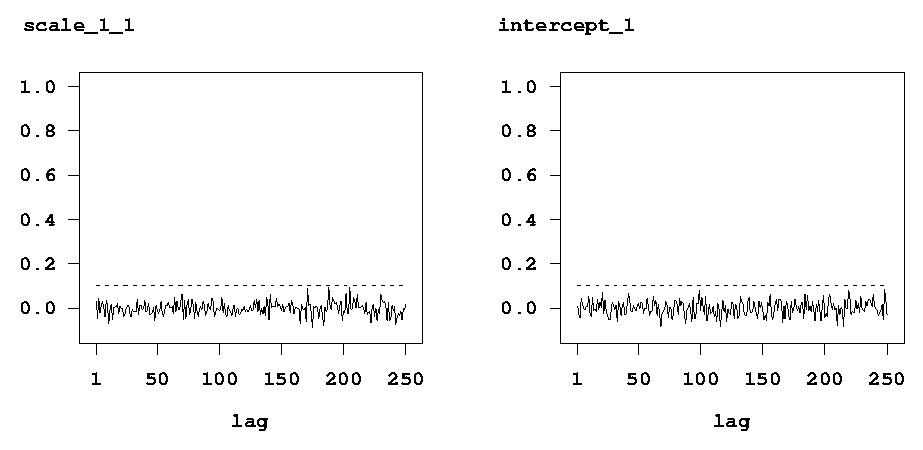
\epsfig{file=grafiken/autocor1.eps,scale=0.75}
{\it\caption{Autocorrelation function for the scale parameter and
the intercept.\label{autocor1}}}
\end{center}
\end{figure}

#> b.plotautocor, mean#

leads to the computation of only the minimum, mean and maximum
autocorrelation functions. The result for the scale parameter is
shown in Figure \ref{autocor2}.

\begin{figure}[ht]
\begin{center}
\epsfig{file=grafiken/autocormean1.ps,scale=0.5}
{\it\caption{Minimum, mean and maximum autocorrelation function
for the scale parameter.\label{autocor2}}}
\end{center}
\end{figure}

Note, that executing the #plotautocor# command also stores the
computed autocorrelation functions in a file named #autocor.raw#
in the output directory of the {\it bayesreg object}.

To save memory, the sampling paths of the estimated parameters are
only stored temporarily by default and will be destroyed, when the
corresponding {\em bayesreg object} is deleted. If we want to
store the sampling paths permanently, we have to execute the
#getsample# command

#> b.getsample#

which stores the sampled parameters in ASCII files in the output
directory. To avoid too large files, the samples are typically
partitioned into several files. Executing the #getsample# command
also produces {\em ps files} of the sampling paths in the output
directory (compare Figure \ref{sample1} for the content of one of
these files).

\begin{figure}[ht]
\begin{center}
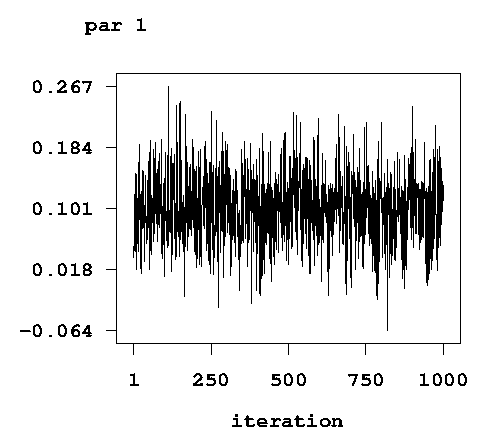
\epsfig{file=grafiken/intercept_sample.eps,scale=0.75}
%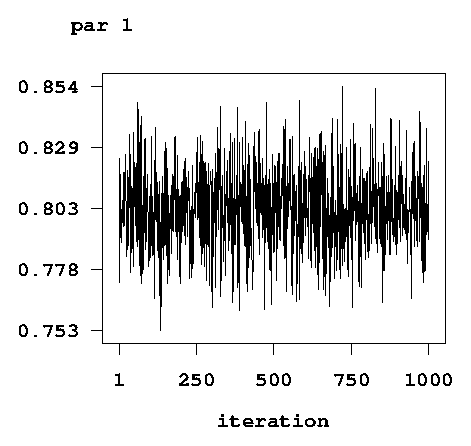
\epsfig{file=grafiken/scale_sample.eps,scale=0.5}
{\it\caption{Sampling path of the intercept.\label{sample1}}}
\end{center}
\end{figure}

\section{Sensitivity analysis}\label{sensitivity}

In some situations the estimation results of a full Bayesian
semiparametric regression model depend on the choice of
hyperparameters, e.g. the parameters $a$ and $b$ defining the
inverse gamma prior of the variances of nonparametric and spatial
effects, it is often recommended to check how sensitive the
results are with respect to changes in the hyperparameters. In the
following we will re-estimate the model from section
\ref{regression} with different choices for the hyperparameters
$a$ and $b$ for each effect in the model. The standard choices for
$a$ and $b$ are $a=b=0.001$. As a first trial we choose a smaller
value for $a$ and $b$:

\begin{verbatim}
> b.regress hazstd = rcw + edu1 + edu2 + tpr + sex
  + bmi(psplinerw2,a=0.00001,b=0.00001) + agc(psplinerw2,a=0.00001,b=0.00001)
  + district(spatial,map=m,a=0.00001,b=0.00001)
  + district(random,a=0.00001,b=0.00001), family=gaussian iterations=12000
  burnin=2000 step=10 predict using d
\end{verbatim}

Figure \ref{sensi1} shows the results for the nonparametric
effects with this choice of hyperparameters. Obviously, the
estimated functions are somewhat smoother but they do not differ
that much from the estimates with the standard choices.

\begin{figure}[ht]
\begin{center}
\epsfig{file=grafiken/f_bmi7.ps,scale=0.5}
\epsfig{file=grafiken/f_age3.ps,scale=0.5} {\it\caption{Results for
the nonparametric effects with hyperparameters $a=b=0.00001$ for
nonparametric and spatial effects.\label{sensi1}}}
\end{center}
\end{figure}

Now we try two further choices for the hyperparameters, each with
$a=1$ and $b$ small. We estimate models with $b=0.005$ and
$b=0.00005$:

\begin{verbatim}
> b.regress hazstd = rcw + edu1 + edu2 + tpr + sex + bmi(psplinerw2,a=1,b=0.005)
  + agc(psplinerw2,a=1,b=0.005) + district(spatial,map=m,a=1,b=0.005)
  + district(random,a=1,b=0.005), family=gaussian iterations=12000 burnin=2000
  step=10 predict using d
\end{verbatim}

\begin{verbatim}
> b.regress hazstd = rcw + edu1 + edu2 + tpr + sex + bmi(psplinerw2,a=1,b=0.00005)
  + agc(psplinerw2,a=1,b=0.00005) + district(spatial,map=m,a=1,b=0.00005)
  + district(random,a=1,b=0.00005), family=gaussian iterations=12000 burnin=2000
  step=10 predict using d
\end{verbatim}

Figure \ref{sensi2} and \ref{sensi3} contain the results for the
nonparametric effects for the two choices of hyperparameters.

\begin{figure}[ht]
\begin{center}
\epsfig{file=grafiken/f_bmi8.ps,scale=0.5}
\epsfig{file=grafiken/f_age4.ps,scale=0.5} {\it\caption{Results for
the nonparametric effects with hyperparameters $a=1$ and $b=0.005$
for nonparametric and spatial effects.\label{sensi2}}}
\end{center}
\end{figure}

\begin{figure}[ht]
\begin{center}
\epsfig{file=grafiken/f_bmi9.ps,scale=0.5}
\epsfig{file=grafiken/f_age5.ps,scale=0.5} {\it\caption{Results for
the nonparametric effects with hyperparameters $a=1$ and $b=0.00005$
for nonparametric and spatial effects.\label{sensi3}}}
\end{center}
\end{figure}

\addcontentsline{toc}{section}{References}

\begin{thebibliography}{99}

\harvarditem{Brezger and Lang}{2005}{brelan05} Brezger, A. and Lang,
S., 2005: Generalized structured additive regression based on
Bayesian P-splines. {\it Computational Statistics and Data
Analysis}, to appear.

\harvarditem{Fahrmeir and Hennerfeind}{2003}{fahhen03} Fahrmeir,
L. and Hennerfeind, A., 2003: Nonparametric Bayesian hazard rate
models based on penalized splines. SFB 386 Discussion paper 361,
University of Munich.

\harvarditem{Fahrmeir et~al.}{2004}{fahkne04} Fahrmeir, L., Kneib,
T. and Lang, S., 2004: Penalized structured additive regression for
space-time data: A Bayesian perspective, {\it Statistica Sinica},
14, 731-761 .

\harvarditem{Fahrmeir and Lang}{2001a}{fahlan01a} Fahrmeir, L. and
Lang, S., 2001a: Bayesian Inference for Generalized Additive Mixed
Models Based on Markov Random Field Priors. {\it Journal of the
Royal Statistical Society C}, 50, 201-220.

\harvarditem{Fahrmeir and Lang}{2001b}{fahlan01b} Fahrmeir, L. and
Lang, S., 2001: Bayesian Semiparametric Regression Analysis of
Multicategorical Time-Space Data. {\it Annals of the Institute of
Statistical Mathematics}, 53, 10-30

\harvarditem{Fahrmeir and Osuna}{2003}{fahosu03} Fahrmeir, L. and
Osuna, L. (2003), Structured count data regression. SFB 386
Discussion paper 334, University of Munich.

\harvarditem{George and Liu}{1981}{geoliu81} George, A. and Liu,
J.W. 1981: {\it Computer Solution of Large Sparse Positive
Definite Systems}, Prentice--Hall.

\harvarditem{Hennerfeind et al.}{2003}{henfah03} Hennerfeind, A.,
Brezger, A. and Fahrmeir, L., 2003: Geoadditive survival models.
SFB Discussion paper 333, University of Munich.

\harvarditem{Kandala et. al}{2001}{kanlan01} Kandala, N. B., Lang,
S., Klasen, S. and Fahrmeir, L. (2001): Semiparametric Analysis of
the Socio-Demographic and Spatial Determinants of Undernutrition
in Two African Countries. {\it Research in Official Statistics},
1, 81-100.

\harvarditem{Lang and Brezger}{2004}{lanbre04} Lang, S. and Brezger,
A., 2004: Bayesian P-splines. {\it Journal of Computational and
Graphical Statistics}, 13, 183-212.

\harvarditem{Spiegelhalter et. al.}{2002}{spibes02} Spiegelhalter,
D.J., Best, N.G., Carlin, B.P. and van der Linde, A. (2002):
Bayesian measures of model complexity and fit. {\it Journal of the
Royal Statistical Society B}, 65, 583-639

\end{thebibliography}


\end{document}
